\documentclass[titlepage]{article}
\usepackage{PreambleCommon}
\usepackage{minted}


\title{Assignment 8: AVL Trees \\[5pt] Part 2: AVL Tree Testing \\[8pt] CS3305/W01 Data Structures}
\author{Casey Hampson}

\begin{document}
\maketitle

\section*{Assignment Description}
This assignment is super vague, so I will explain what I did and why I did it here. We are asked to confirm that the \mintinline{java}|AVLTree| class from the book spits out a valid AVL tree. An AVL tree is a binary search tree that is well balanced, meaning that all of its nodes have a balance factor, call it $b$, such that $\abs{b} < 2$.

So, we need to test that 1) the tree it spits out is a binary search tree, and 2) that the tree is well balanced. If we can do that for three test cases (which I just will just randomly generate), then I think that should satisfy the requirements for this assignment. I choose to test only integers because there is no loss of generality compared to choosing any other comparable type.

To test if it is a binary search tree, we need to check that for each node, its left child's value is less and its right child's value is greater than its own value. To test if it is balanced, we can simply iterate through all the nodes and check to make sure that each node's balance factor is less than 2 and greater than -2.


\section*{Program Output}
\begin{center}
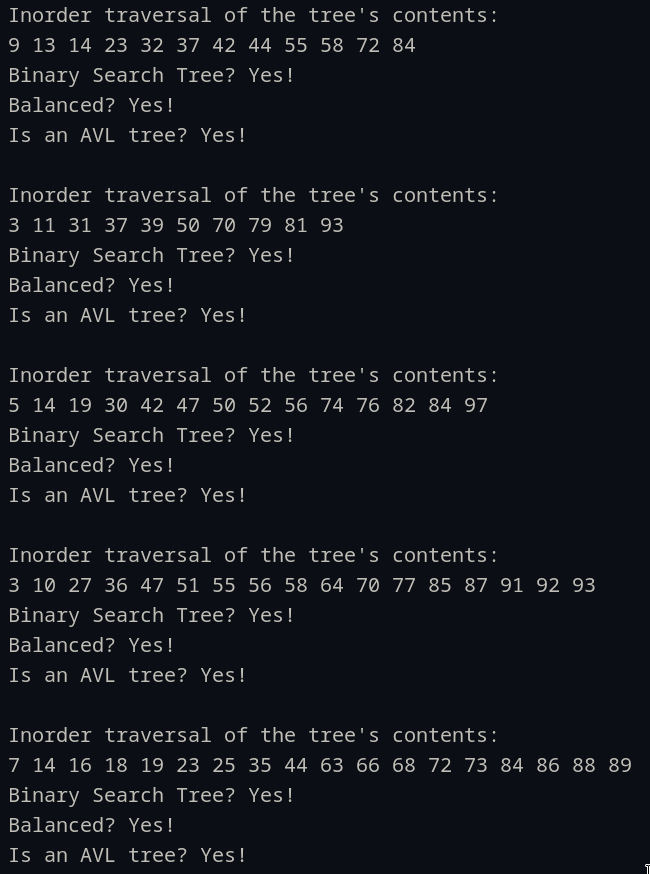
\includegraphics[width=0.7\linewidth]{./res/1.png}
\end{center}


\pagebreak
\section*{Source Code}
\inputminted{java}{./P2.java}




\end{document}
